\documentclass[a4]{article}
\usepackage{url}
\usepackage{epsfig}
\usepackage{tabularx}

\bibliographystyle{unsrt}
\emergencystretch 2in

\title{JSAV: JavaScript Sequence Alignment Viewer}
\date{18th September, 2014}
\author{Andrew C. R. Martin\mbox{${}^{\rm a}$}\footnote{to whom
    correspondence should be addressed}\\
    \mbox{${}^{\rm a}$}Institute of Structural and Molecular Biology,\\
Division of Biosciences, University College London,\\
Darwin Building, Gower Street,\\
London WC1E 6BT}

\begin{document}
\maketitle

\begin{abstract}
\noindent{\bfseries Summary:} The JavaScript Sequence Alignment Viewer
(JSAV) is designed as a simple-to-use JavaScript component for
displaying sequence alignments on web pages.  The display of sequences
is highly configurable with options to allow alternative colouring
schemes, sorting of sequences and `dotifying' repeated amino acids. An
option is also available to submit selected sequences to another web
site, or to other JavaScript code.  \\
\noindent{\bfseries Availability and Implementation:} 
JSAV is implemented purely in JavaScript making use of the JQuery and
JQuery-UI libraries. It does not use any HTML5 specific options to help with
browser compatibility. The code is documented using JSDOC
and is available from \url{http://www.bioinf.org.uk/software/jsav/}\\
\noindent{\bfseries Contact:} andrew@bioinf.org.uk --or--
andrew.martin@ucl.ac.uk
\end{abstract}


%%%%%%%%%%%%%%%%%%%%%%%%%%%%%%%%%%%%%%%%%%%%%%%%%%%%%%%%%%%%%%%%%%%%
\section{Introduction}
Viewing multiple sequence alignments (MSAs) is a fundamental
requirement in analysis of protein sequences, allowing us to visualize
conservation across protein families as well as unusual features of
particular sequences. As a result, there are a plethora of tools for
viewing MSAs. These range from tools which provide attractive printed
output, through (operating-system dependent, or independent)
standalone tools, to web-based viewers.

Two of the earliest tools were HOMED\cite{stockwell:homed} and
MALIGNED\cite{clark:maligned} written for VAX/VMS workstations.
Neither seems to be actively maintained or easily available any
more. Other early viewers include GeneDoc\cite{nicholas:genedoc},
BioEdit, Seaview\cite{galtier:seaview} and DCSE\cite{derijk:dcse}
which is part of the RnaViz package for visualizing RNA secondary
structure\cite{derijk:rnaviz}, but which can be used for protein
sequence alignments.  A problem in writing graphical software is the
operating-system dependency of many graphics libraries.
CINEMA\cite{parrysmith:cinema} was probably the first sequence
alignment viewer and editor implemented in Java, a platform
independent programming language allowing graphical user interfaces
(GUIs) to run on any operating system. It has now been rewritten in
C++ and is part of UTOPIA\cite{pettifer:utopia}. Other software
includes MPSA\cite{blanchet:mpsa}, ANTHEPROT\cite{deleage:antheprot}
and ClustalX\cite{thompson:clustalx}, a GUI for the ClustalW multiple
sequence alignment program, providing an integrated environment for
aligning sequences and analyzing results. Clustal Omega is the most
recent version, but at the time of writing only has a command line
interface --- a beta version of a GUI is due to be released soon.

More recent developments include the Protein Family Alignment
Annotation Tool (PFAAT)\cite{johnson:pfaat} designed specifically for
family analysis and incorporating residue annotation tools as well as
integration with Jmol for protein structure display. Like early
versions of CINEMA, PFAAT is implemented in Java for operating system
independence. CLC~Viewer is a recent free package written in Java
which contains a number of integrated tools and acts as a core product
for adding other features through a commercial version.  A more
complete list of MSA viewers is available on the web at
\url{http://en.wikipedia.org/wiki/List_of_alignment_visualization_software}.

Probably the most popular of the available tools is
Jalview\cite{clamp:jalview} which is available in two versions: a
standalone Java application which provides many tools and facilities,
and as a `light' version (JalviewLight) --- a Java applet that can be
embedded in a web page. The latter responds to the need for web site
developers to be able to embed MSA visualization.

However, in recent years there has been a gradual move away from using
Java applets in web development. New HTML features such as the HTML5
Canvas, and powerful JavaScript libraries such as Bootstrap, JQuery
and JQuery-UI that provide an easier syntax for accessing elements of
a web page together with new widgets such as sliders and drag-and-drop
support, have overtaken Java as the method of choice for creating
interactive web sites with complex requirements.  Such features are
used widely by popular web sites such as Google Mail, Google Docs and
Facebook.  Recently the Jmol structure viewer has been reimplemented
in JavaScript as JSmol.

Consequently, over the last couple of years a small number of
JavaScript-based sequence alignment viewers have started to be
developed. These include MODalign\cite{barbato:modalign},
Alignment-Annotator\cite{gille:2014aa}, SnipViz\cite{jaschob:2014},
and `Sequence', a component of the BioJS library\cite{gomez:2014}.

MODalign is part of the MODexplorer package\cite{kosinski:2013}, a web
site for protein modelling, but does not appear to be available as a
download for use in other web sites. 

Alignment-Editor is part of a more complex system, STRAP. STRAP uses a
Java server-side interpreter, Alignment-to-HTML\cite{gille:2014},
which parses the STRAP scripting language and create an alignment in a
form that can be rendered in Web browsers. The server-side element
allows tasks such as sequence retrieval, computation of alignments and
communication with BioDAS-servers. The rendering system includes a
selection of colouring schemes, highlighting of conserved and variable
positions in the alignment, reordering and deletion of sequence by
drag-and-drop, and residue annotation as well as links to 3D
visualization and sequence groups. It exploits JavaScript and HTML5
using the HTML5 canvas to draw helices and other visual elements.  The
description of Alignment-Editor\cite{gille:2014aa} suggests that
alignments should be prepared using the full Java system and the final
alignment can then be downloaded as HTML files in a ZIP archive. The
software is licenced under the GPL and available from the authors on
request, but the JavaScript visualizer doesn't apperar to be available
by itself. While in principle possible, no simple documentation is
provided to enable the client-side JavaScript/HTML5 viewer to be used
without the server side software.

SnipViz is a compact and lightweight component designed for display 
of multiple versions of gene and protein sequences ---
i.e.\ essentially identical sequences with mutations.
It provides a very simple clean display focused around both DNA and
protein sequences allowing very long sequences through a scrolling
mechanism which also shows a small box on a representation of the
complete sequence to show the relative position within the complete
alignment.  It also allows display of phylogenetic trees stored in
Newick format.

`Sequence', is a BioJS component for visualizing sequences. It
Only very simple views though flexible highlighting



Sequence \ldots.
In addition, there is an intention to port JalviewLight to
JavaScript.

JSAV (JavaScript Sequence Alignment Viewer) is a novel JavaScript
component that adds to this list. The primary motivation for
implementing a new tool was the need for a tool with the following
requirements: (i)~a very simple-to-use lightweight component that can
easily be dropped into a web site; (ii)~provision of flexible
colouring schemes and `dotifying' alignments (replacing repeated
residues with dots); (iii)~the ability to sort sequences --- both
complete sequences or regions of sequences; (iii)~the ability to
remove sequences from the alignment; (iv)~the ability to highlight
regions in the alignment; (v)~the ability to export a selected set of
sequences in FASTA format; (vi)~the ability to submit a selected set
of sequences to another web site or to local JavaScipt code.



%%%%%%%%%%%%%%%%%%%%%%%%%%%%%%%%%%%%%%%%%%%%%%%%%%%%%%%%%%%%%%%%%%%%
\section{Implementation}

\begin{figure}
\footnotesize
\begin{verbatim}
var MySeqs = Array();
MySeqs.push({ id :"id1b1.L",  
   sequence :"SASSSVNYMYACREFGHIKLMNPTRSTVWY"});
MySeqs.push({ id :"id1a.L",   
   sequence :"SASSSTNYMYACDEFGHIKLMNPQRSTVWY"});
MySeqs.push({ id :"id2b1.L",  
   sequence :"SASSTCNYMTACDEEGHIKLMNP-RSTCWY"});

var MyOptions = Array();
MyOptions.sortable = true;
MyOptions.selectable = true;
MyOptions.deletable = true;
MyOptions.toggleDotify = true;
MyOptions.toggleNocolour = true;
MyOptions.consensus = true;
MyOptions.selectColour = true;

printJSAV('sequenceDisplay', MySeqs, MyOptions);
\end{verbatim}
\caption{\label{fig:code}Example code to create a
JavaScript array of sequence objects, set options and 
create the alignment viewer.}
\end{figure}

\begin{figure}
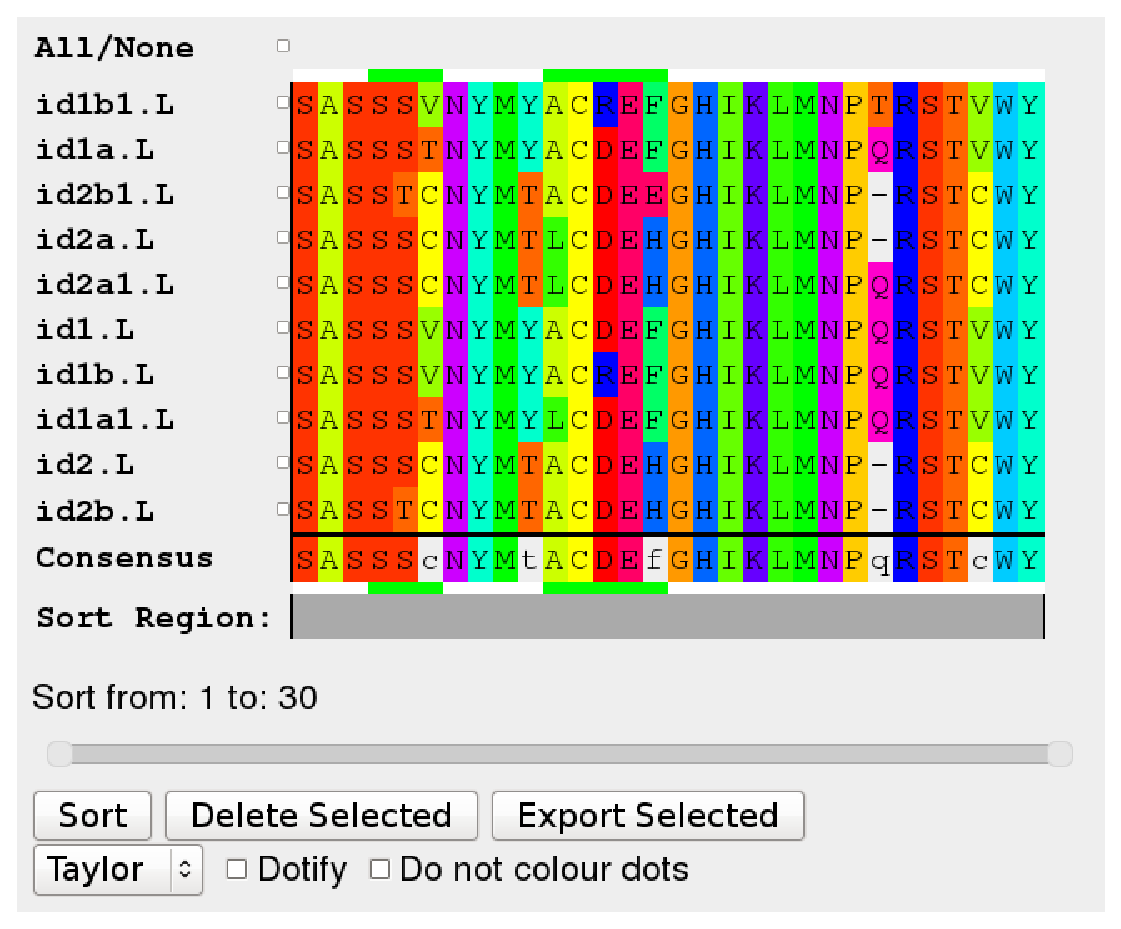
\epsfig{file=demo.eps,width=\columnwidth}
\caption{\label{fig:demo}A typical JSAV alignment view}
\end{figure}

%JSAV is implemented purely in JavaScript. JSAV employs the JQuery
%library to ease access to elements of the HTML that it generates and
%uses JQuery-UI to implement a two-value slider that is used to specify
%a range of positions in the alignment.

JSAV is implemented purely in JavaScript employing the JQuery and
JQuery-UI libraries. As input, the code requires an array of
JavaScript objects which contain two elements: a unique identifier for
a sequence and the sequence itself --- all sequences must be
pre-aligned.  Secondly a set of options can be provided. These control
the display and facilities available to the end user of a web site to
modify the view of the MSA.  A brief extract of sample code is shown
in Fig~\ref{fig:code} with the results shown in Fig~\ref{fig:demo}.

The end-user can sort the sequences --- the code selects the most
representative sequence, displaying that at the top of the alignment
followed by the most similar sequence and so on. By default, sorting
is performed across the whole sequence, but a two-handled slider
allows the range of positions on which the sort is based to be
modified. Different colouring schemes are available duplicating those
provided in Jalview. The alignment can also be `dotified', replacing
residues repeated between sequences with dots in order to emphasize
amino acid differences. Colouring of dotified residues can also be
switched off or on. Sequences can be selected and deleted from the
alignment; a consensus sequence can be displayed at the bottom of the
alignment and updates automatically when sequences are deleted. The
complete set of sequences, or a selected subset, can be submitted to
another web site, or passed to another JavaScript function for
integration with other tools. Tooltips are provided for each option
and all options are documented in detail on the web site. The number
and size of sequences in the MSA is limited only by the memory
available to the web browser.

%%%%%%%%%%%%%%%%%%%%%%%%%%%%%%%%%%%%%%%%%%%%%%%%%%%%%%%%%%%%%%%%%%%%
\section{Availability}
The software may be downloaded from
\url{http://www.bioinf.org.uk/software/jsav/} where demonstrations,
including the ability to upload your own MSA, are available together
with full documentation implemented with JSDOC.

\bibliography{jsav}

\end{document}
